\documentclass[serif]{beamer}
\usepackage[english]{babel}
\usepackage[utf8]{inputenc}
\usepackage[T1]{fontenc}
\usepackage{palatino}
\usepackage{url}
\usetheme{PaloAlto}
\useoutertheme{infolines}
\usepackage{amsmath}
\usepackage{mathrsfs}
\usepackage{multirow}
\usepackage{natbib}
\usepackage{tabularx}
\usepackage{listings}

\newcommand{\newblock}{}
\renewcommand\figurename{Figura}
\renewcommand\tablename{Tabla}
%\renewcommand{\fnum@figure}[1]{\textbf{Figura~\thefigure. }}
%\renewcommand{\fnum@table}[1]{Tabla~\thetable. }

\usecolortheme{beaver}
\logo{
\includegraphics[height=0.7cm]{logoCinvestavGris}}
\graphicspath{{images/}}
%%%%%%%%%
\usepackage{graphicx}
\usepackage{etex}
\reserveinserts{100}
\usepackage{morefloats}
\usepackage{dcolumn}
\usepackage{array}
\usepackage{chngpage}
\usepackage{verbatim}
\usepackage{moreverb}
%\decimalpoint
\let\verbatiminput=\verbatimtabinput
\def\verbatimtabsize{4\relax}
\newcolumntype{K}{>{\centering\arraybackslash$}X<{$}}


%%%%%%%%%%%%%%%%%%%%%%%%%%%%%%%%%%%%%%%%%%%%%%%%%%%%%%%%%%%%%%%%%%%%%%%%%%%%%%%%%
\title[mocDE]{Evolución Diferencial Compacta Multi-Objetivo}
\author[Moisés \textsc{Osorio}]{Jesús Moisés \textsc{Osorio Velázquez} \linebreak Dr. Carlos A. \textsc{Coello Coello} }
\date{Abril 16, 2012}
\institute[\textsc{CINVESTAV-IPN}]{\textsc{Centro de Investigación y de Estudios Avanzados del IPN}}


\begin{document}

%\setbeamertemplate{background}{\includegraphics[height=96mm,width=128mm]{Images/Background/background}}
\frame{
  \titlepage
}
\setbeamertemplate{background}{}

\frame[allowframebreaks]{
	\setcounter{tocdepth}{2}
	\tableofcontents
}

\section{Introducción}

\subsection{Problema}
\begin{frame}
\frametitle{\insertsubsection}
	\begin{center}
	\emph{Diseñar e implementar un algoritmo evolutivo multiobjetivo no poblacional que haga uso de menos recursos de cómputo que los algoritmos del estado del arte}
	\end{center}
\end{frame}

\subsection{Objetivos}
\begin{frame}
\frametitle{\insertsubsection}
	\begin{itemize}\setlength{\itemsep}{4mm}
		\item Obtener resultados competitivos con respecto a los algoritmos representativos del estado del arte
		\item Ser compacto y utilizar menos recursos computacionales que los algoritmos representativos del estado del arte
	\end{itemize}
\end{frame}


\section{Teoría}

\subsection{Introducción}
\begin{frame}
La optimizaci\'{o}n se define como el proceso para minimizar, o maximizar, el valor de una o varias funciones que representan los objetivos de un problema. Cuando se habla de dos o m\'{a}s funciones objetivo, se trata de optimizaci\'{o}n multiobjetivo.

De manera formal, un problema de optimizaci\'{o}n es expresado como
\begin{align}
\displaystyle \min_{\vec{x} \in X} \vec{f} (\vec{x})
\end{align}
donde $\vec{f} : \mathbb{R}^n \rightarrow \mathbb{R}^k$ es el vector de funciones objetivo, $\vec{x} \in \mathbb{R}^n$ es el vector de variables de decisi\'{o}n y $X \subseteq \mathbb{R}^n$ es el espacio de b\'{u}squeda.
\end{frame}
\begin{frame}
En un problema de optimizaci\'{o}n multiobjetivo (POM), normalmente se utiliza la \emph{dominancia de Pareto} para comparar soluciones. La dominancia de Pareto fue originalmente propuesta por Francis Ysidro Edgeworth y, posteriormente, fue generalizada por Vilfredo Pareto. Bajo la dominancia de Pareto, se dice que una soluci\'{o}n $\vec{x_1} \in X$ domina a (es mejor que) $\vec{x_2} \in X$ ($\vec{x_1} \prec \vec{x_2}$) si y solo si
\begin{align}
\forall i \in \{1,..,k\} \qquad f_i(\vec{x_1}) \leq f_i(\vec{x_2}) \\ 
\exists i \in \{1,..,k\} \qquad f_i(\vec{x_1}) < f_i(\vec{x_2})
\end{align}
La dominancia de Pareto no impone un orden total en $\mathbb{R}^k$ ya que algunas soluciones pueden resultar incomparables. Por lo tanto, la mayor\'{i}a de los POMs no tienen una soluci\'{o}n \'{u}nica, sino un conjunto de ellas.
\end{frame}
\begin{frame}
En un POM, el \emph{conjunto de \'{o}ptimos de Pareto} $\mathcal{P}$ es definido como
\begin{align}
\mathcal{P} = \{ \vec{x*} \in X | \forall \vec{y} \in X \quad \vec{y} \npreceq \vec{x*} \}
\end{align}

El \emph{frente de Pareto} de un POM es definido, a partir de su conjunto de \'{o}ptimos de Pareto, de la siguiente manera
\begin{align}
PF = \{ \vec{u} = (f_1(\vec{x}),...,f_k(\vec{x})) | \vec{x} \in \mathcal{P} \}
\end{align}
\end{frame}
\begin{frame}
De esta manera, cuando un algoritmo utiliza la dominancia de Pareto para comparar soluciones, tiene como objetivo al resolver un POM, encontrar $\mathcal{P}$ y su correspondiente frente de Pareto. Ya que las soluciones a reportar por un algoritmo son finitas, aumenta la importancia de mantener una distribuci\'{o}n entre dichos resultados. Dicha distribuci\'{o}n, mas la convergencia de los resultados, se vuelven los indicadores m\'{a}s importantes sobre la calidad de las soluciones reportadas por un algoritmo multiobjetivo.
\end{frame}


\subsection{Evolución Diferencial (DE)}

\subsubsection{Descripción}
\begin{frame}
\frametitle{\insertsubsubsection}
	\begin{itemize}\setlength{\itemsep}{4mm}
		\item Algoritmo de optimización estocástico y poblacional
		\item Creada por Storn y Price en 1996
		\item Desarrollada para optimizar funciones reales
		\item Requiere pocas variables de control
		\item Es robusto y fácil de usar
	\end{itemize}
\end{frame}

\subsubsection{Mecanismo}
\begin{frame}
\frametitle{\insertsubsubsection}
	\vspace*{-0.2cm}
	\begin{figure}
	\centering
	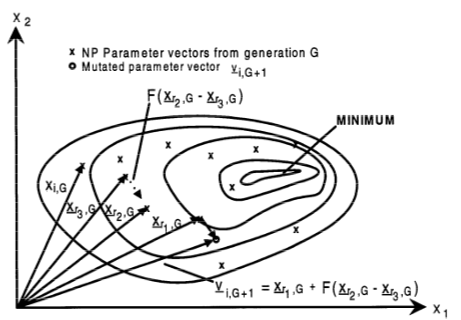
\includegraphics[width=0.8\textwidth]{de.png}
	\caption{Ejemplo de una función de costo bidimensional donde se muestra la forma de generar $v_i,G+1$}
	\end{figure}
\end{frame}

\subsubsection{Algoritmo}
\begin{frame}
\frametitle{\insertsubsubsection}
	\vspace*{-0.2cm}
	\begin{figure}
	\centering
	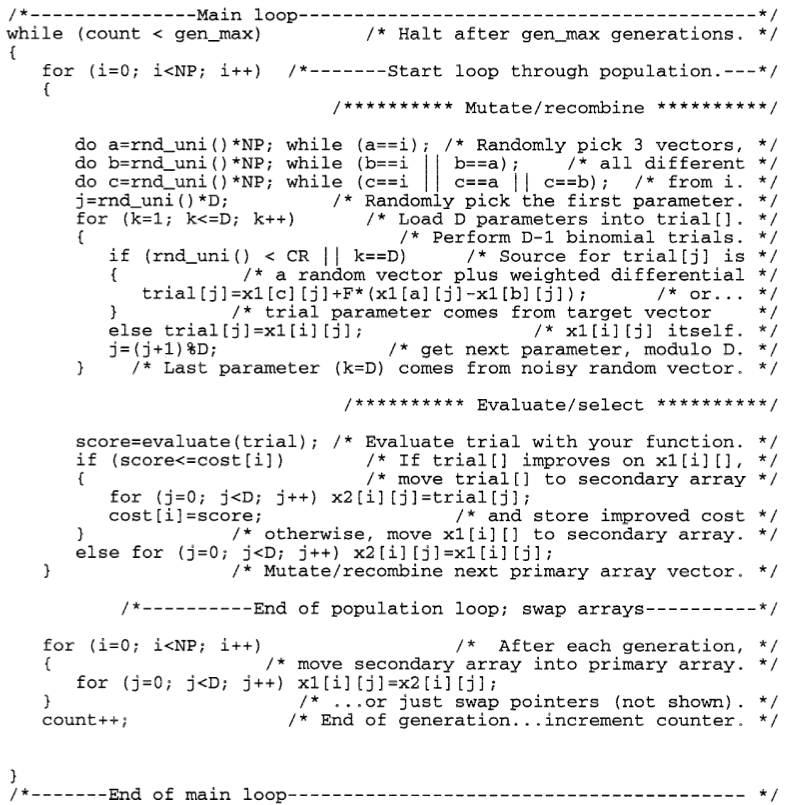
\includegraphics[height=0.9\textheight]{de_algorithm.png}
	\caption{DE en 19 líneas de código en C}
	\end{figure}
\end{frame}

\subsection{Evolución Diferencial Compacta (cDE)}

\subsubsection{Descripción}
\begin{frame}
\frametitle{\insertsubsubsection}
	\begin{itemize}\setlength{\itemsep}{4mm}
		\item Pertenece a la clase de Algoritmos de Estimación de la Distribución
		\item No utiliza una población de individuos
		\item Utiliza una representación estadística de la población
		\item Este enfoque es necesario para resolver problemas de optimización complejos cuando no se cuenta con mucho poder computacional
	\end{itemize}
\end{frame}

\subsubsection{Algoritmo}
\begin{frame}
\frametitle{\insertsubsection}
	\vspace*{-0.2cm}
	\begin{figure}
	\centering
	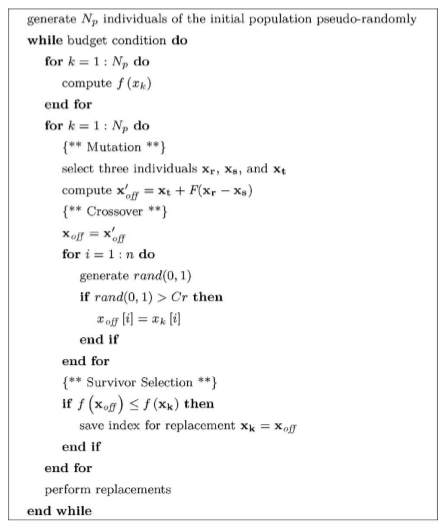
\includegraphics[height=0.9\textheight]{cde_algorithm.png}
	\caption{Pseudocódigo de cDE/rand/1/bin}
	\end{figure}
\end{frame}

\section{Estado del Arte}

\subsection{Pareto Archived Evolution Strategy (PAES)}
\subsubsection{Descripción}
\begin{frame}
\frametitle{\insertsubsubsection}
	\begin{itemize}\setlength{\itemsep}{4mm}
		\item Consiste de una estrategia evolutiva (1+1)
		\item Utiliza un archivo externo donde almacena las soluciones no dominadas encontradas durante el proceso de optimización
		\item Posee una malla adaptable que divide el espacio objetivo de manera recursiva, permitiendo calcular el grado de densidad en el que se encuentran las soluciones
		\item Obtiene resultados no muy competitivos, pero es el mejor algoritmo no poblacional
	\end{itemize}
\end{frame}

\subsubsection{Algoritmo}
\begin{frame}
\frametitle{\insertsubsubsection}
	\vspace*{-0.2cm}
	\begin{figure}
	\centering
	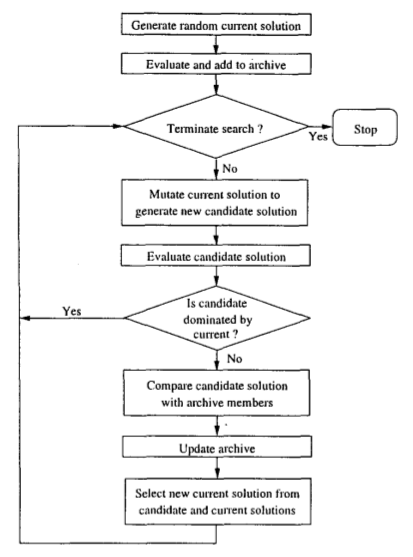
\includegraphics[height=0.9\textheight]{paes1.png}
	\caption{Algoritmo de PAES}
	\end{figure}
\end{frame}

\begin{frame}
\frametitle{\insertsubsubsection}
	\vspace*{-0.2cm}
	\begin{figure}
	\centering
	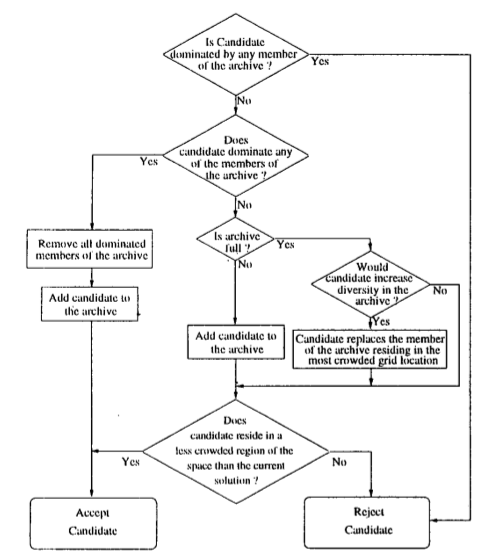
\includegraphics[height=0.9\textheight]{paes2.png}
	\caption{Algoritmo de la malla utilizada por PAES}
	\end{figure}
\end{frame}

	
\subsection{MOEA/D}
\subsubsection{Descripción}
\begin{frame}
\frametitle{\insertsubsubsection}
	\begin{itemize}\setlength{\itemsep}{4mm}
		\item Descompone el problema en $p$ subproblemas escalares
		\item Aplica una escalarización de Chebyshev
		\item Optimiza los subproblemas de forma simultánea
		\item Incorpora un método de detección de subproblemas difíciles
		\item Ganador de la competencia CEC’09 MOEA
	\end{itemize}
\end{frame}

\subsection{NSGA-II}
\subsubsection{Descripción}
\begin{frame}
\frametitle{\insertsubsubsection}
	\begin{itemize}\setlength{\itemsep}{4mm}
		\item Estima la densidad de la población con su \emph{Crowding Distance}
		\item Utiliza un comparador que se basa en su \emph{Crowding Distance} y el \emph{Non-domination Rank}
		\item Su desempeño se degrada rápidamente al aumentar los objetivos del problema
	\end{itemize}
\end{frame}

\begin{frame}
\frametitle{\insertsubsubsection}
	\vspace*{-0.2cm}
	\begin{figure}
	\centering
	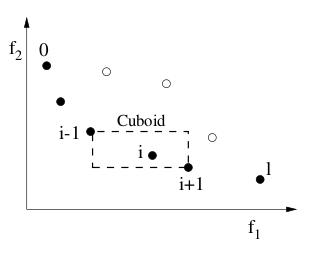
\includegraphics[width=0.6\textwidth]{crowdingdistance.png}
	\caption{Cómputo de \emph{Crowding Distance}}
	\end{figure}
\end{frame}


\section{mocDE}

\subsection{Actividades}
\begin{frame}[allowframebreaks]
\frametitle{\insertsubsection}
	\begin{enumerate}
		\item Revisión del estado del arte y literatura relacionada. Obtener un panorama amplio del trabajo pasado y actual sobre la optimización multiobjetivo, a fin de compararse y mejorar, de algún modo, dichos trabajos.
		\item Diseño general del algoritmo principal. Definir de manera general, el enfoque de solución a utilizar.
		\item Implementación básica capaz de resolver problemas sencillos. Implementar una versión del algoritmo que sea competitiva en problemas generalmente reconocidos como fáciles.
		\item Redacción del protocolo de tesis. Definir el problema, el alcance del trabajo de investigación y el plan general de trabajo.
		\item Implementación de scripts de pruebas y estadísticos. Implementar scripts que permitan obtener valores estadísticos sobre el desempeño del algoritmo, a fin de ser comparado con el estado del arte.
		\item Mejora de la convergencia de la implementación básica. Mejorar la convergencia de los resultados obtenidos por el algoritmo, a fin de que sea competitivo en problemas más difíciles que aquéllos resueltos por la versión básica.
		\item Mejora de la distribución de la implementación mejorada. Aumentar la distribución de los resultados obtenidos por el algoritmo ya que, como la convergencia, éste es otro indicador de la calidad de los mismos.
		\item Escritura de tesis. Redactar aquellos capítulos que no necesiten de los resultados finales del algoritmo.
		\item Refinamiento general de la implementación del algoritmo. Refinar los ltimos detalles del algoritmo para alcanzar su máxima eficacia y eficiencia.
		\item Finalización de escritura de tesis. Redactar aquellos capítulos finales dependientes de los resultados del algoritmo.
		\item Publicación de resultados. Escribir un artículo en un congreso internacional para dar a conocer los resultados de esta investigación.
	\end{enumerate}
\end{frame}

\begin{frame}
\frametitle{\insertsubsection}
	\vspace*{-0.2cm}
	\begin{figure}
	\centering
	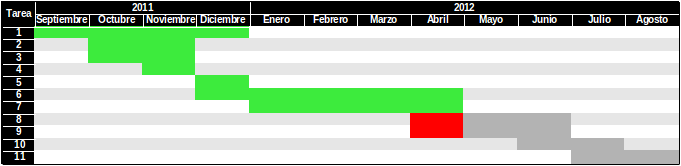
\includegraphics[width=0.7\textwidth]{cronograma.png}
	\caption{Cronograma de actividades}
	\end{figure}
\end{frame}


\subsection{Implementación actual}
\subsubsection{Algoritmo principal}
\begin{frame}[fragile]
\frametitle{\insertsubsubsection}
	Algoritmo principal
	\tiny
	\verbatiminput{mocde-main.code}
\end{frame}


\subsubsection{Algoritmo del archivo de soluciones}
\begin{frame}[fragile]
\frametitle{\insertsubsubsection}
	Archivo de soluciones
	\tiny
	\verbatiminput{mocde-grid.code}
	
	\normalsize
	Escalarización de Chebyshev
	\tiny
	\verbatiminput{mocde-chebyshev.code}
\end{frame}

\subsection{Trabajo actual}
\begin{frame}
\frametitle{\insertsubsubsection}
	\begin{itemize}\setlength{\itemsep}{4mm}
		\item Profundizar en los resultados de las pruebas y su relación con el parámetro $w$ de mocDE.
		\item Comenzar a escribir el trabajo de tesis.
	\end{itemize}
\end{frame}


\subsection{Resultados}
\begin{frame}
\frametitle{\insertsubsection}
	\vspace*{-0.2cm}
		Los parámetros utilizados para las funciones de prueba son los detallados en la tabla \ref{tab:params}. Donde $n$ es el número de variables del problema.
		\tiny
\begin{table}
	\centering
        \begin{tabularx}{1\textwidth}{| c || c | K |}
        \hline
            Algorithm & Parameter & Value \\ \hline \hline
            \multirow{4}{*}{\textbf{mocDE}}
                & Evaluations & 300000 \\
                & Population size & 100 \\
                & Differential variation & 0.9 \\
                & Crossover probability & 0.3 \\
                & Search width & (1 .. 15) \\
                \hline
            \multirow{8}{*}{\textbf{MOEA/D}}
                & Evaluations & 300000 \\
                & Population size & 100 \\
                & Niche size & 100 (2D), 150 (3D) \\
                & Update limit & 10 (2D), 15 (3D) \\
                & Differential variation & 1.0 \\
                & Crossover probability & 0.5 \\
                & Mutation rate & 1.0 / n \\
                & Mating selection probability & 0.9 \\
                \hline
            \multirow{6}{*}{\textbf{PAES}}
                & Evaluations & 300000 \\
                & Archive size & 100 \\
                & Mutation rate & 1.0 / n \\
                & Bisection & 5 \\
                & Distribution index & 20 \\
                \hline
            \multirow{4}{*}{\textbf{NSGA-II}}
                & Evaluations & 300000 \\
                & Population size & 100 \\
                & Mutation rate & 0.01 \\
                & Crossover probability & 0.9 \\
                \hline
        \end{tabularx}
    \caption{\label{tab:params} Algorithm parameters.}
\end{table}
\end{frame}

%RESULTS%

\section*{Referencias}
\begin{frame}[allowframebreaks]
\frametitle{\insertsection}
  \begin{small}
  	\nocite{*}
    \phantomsection
    \bibliographystyle{alpha}
    \bibliography{tesis}
  \end{small}
\end{frame}

\end{document}
